In the current section we present our framework for scalable and NUMA-aware producer-consumer data exchange. 
Our system follows the principle of separating mechanism and policy.
To this end, we consider two independent logical entities: 
\begin{enumerate}
	\item \emph{A single consumer pool (SCPool)} mechanism manages the tasks arriving to a given consumer while introducing the possibility of stealing some tasks by other consumers.
	\item A management policy is responsible for operating SCPools: the policy routes producers' requests to the appropriate consumers and initiates stealing between the pools. This way, the policy controls the system's behavior according to considerations of load-distribution, throughput, fairness, locality, etc.
\end{enumerate} 

\begin{algo}[!ht]
\caption{API for a Single Consumer Pool with stealing support.} 
\label{alg:scpool-api}
\begin{distribalgo}[1]
\scriptsize

\INDENT {\bf SCPool API:}
	\STATE produce(Task) \elcomment {Insert the task to the pool, returns false if no space left in the pool.}
	\STATE produceForce(Task) \elcomment {Inserts the task to the pool, expanding the pool if necessary. }
	\STATE consume() \elcomment {Retrieves a task from the pool, returns $\bot$ if no tasks in the pool are detected.}
	%\STATE getStealingScore() \elcomment {Returns a score corresponding to the amount of tasks to steal.}
	\STATE steal(SCPool from) \elcomment{Tries to steal a number of tasks from the given pool and move them to the current pool. Returns one of the stolen tasks or $\bot$. }%We guarantee that if there are tasks in the \emph{from} pool at the beginning of steal invocation, then either steal function returns a task, or there is another thread that returns a task during the steal execution.}
\ENDINDENT

\end{distribalgo}
\end{algo}


The SCPool API provides the abstraction of a single-consumer task pool with stealing support, see Algorithm~\ref{alg:scpool-api}.
A producer can invoke two types of insertion operations: \emph{produce}, which attempts to insert a task to the given pool and fails if the pool is full, and \emph{produceForce}, which always succeeds by expanding the pool on demand.
There are also two ways to retrieve a task from the pool: the owner of the pool (only) can call the \emph{consume} function; while any other thread can invoke the \emph{steal} function, which tries to transfer a number of tasks between the pools and to return one of the stolen tasks. 
The pool must guarantee the following \emph{stealing property}, which is necessary for system liveness:
\begin{property}
If a pool is not empty at the beginning of the steal operation, then either the steal operation retrieves a task, or another thread retrieves a task during the steal execution.
\end{property}


\begin{figure}[htb]
	\centering
	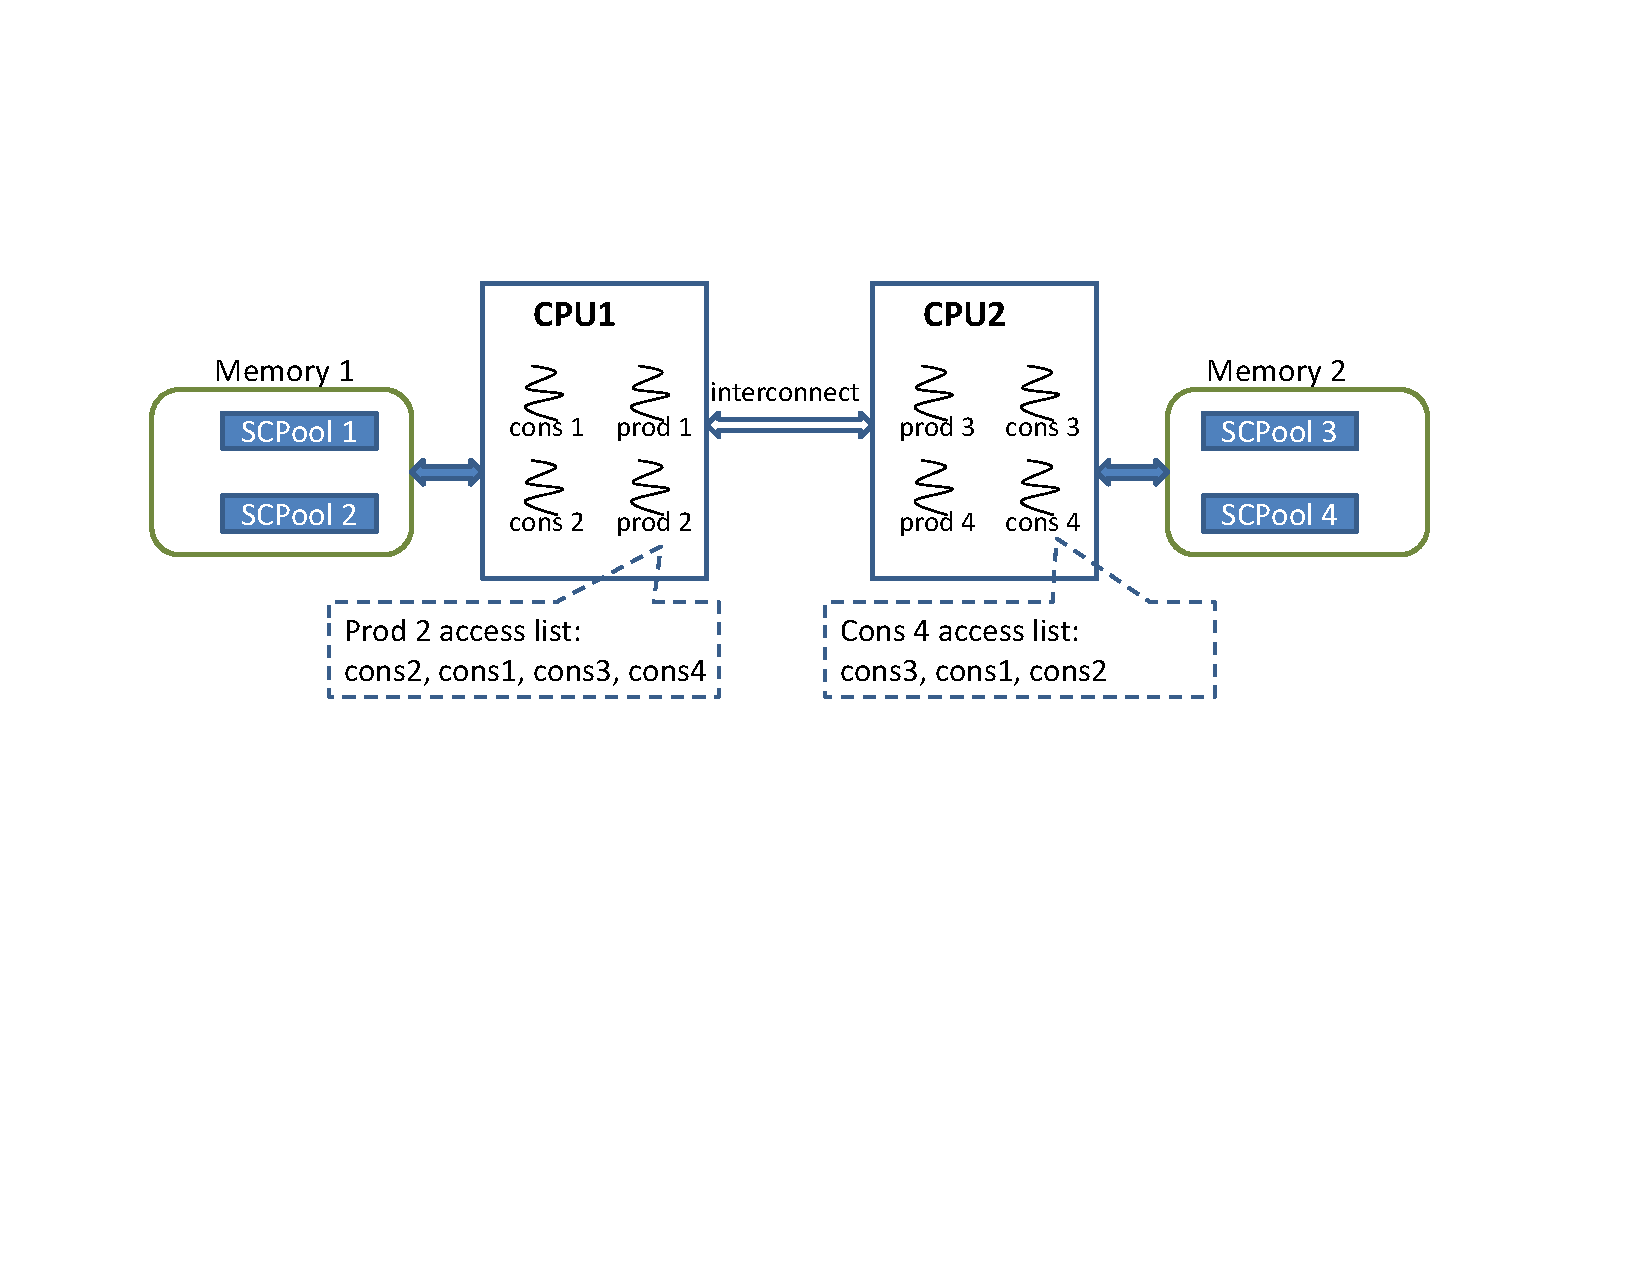
\includegraphics[width=0.7\textwidth]{figures/system-fig}
	\caption{\footnotesize{System overview: process $p_i$ observes a proximity list of available consumers sorted according to their distance from $p_i$. Locality groups are important both for task insertions (insert a task to the closest consumer), and for task stealing (steal a task from the closest consumer).}}
	\label{fig:system-fig}
\end{figure}


As mentioned earlier, an inter-pool communication policy operates the SCPools in a way that is appropriate for the given desired system properties. 
We believe that such a policy is a subject to engineering optimizations and its behavior primarily depends on the specific workloads and demands.
In the current work, we propose a policy for a lock-free starvation-free pool, which exploits the locality properties of NUMA architectures and is aimed for achieving maximal throughput (note that a policy is independent from the underlying SCPool implementations):
\begin{itemize}
	\item {\bf Proximity lists.} The consumers participating in the system are aware of their current processor affinity. This way, each process in the system (producer or consumer) can observe the list of all the consumers sorted according to their distance from that process (see Figure~\ref{fig:system-fig}). Intuitively, we build a system in which a producer mostly interacts with the closest consumer, and the stealing mainly happens inside the same processor node. 
	\item {\bf Producer's policy.} A producer inserting a task first call the \emph{produce} function of the closest SCPool. Note that a produce operation might fail if the pool is full (an evidence of the overload on the corresponding consumer).  In this case, the producer tries to insert a task to other pools, in the order defined by its proximity list. If all the pools are full, then the producer invokes the \emph{produceForce} operation on the closest SCPool, which always succeeds and expands the pool by demand. 
	\item {\bf Consumer's policy.} A consumer works in a loop of consuming the tasks of its own SCPool. If the consumer's SCPool is empty, a consumer tries to steal tasks from other pools in the order defined by its proximity list. 
\end{itemize}



% The inter-pool communication policy is a subject to engineering optimizations and its optimal behavior should probably
% depend on the workload. For the purpose of our evaluation we propose the following approach. 
	% Producer policy. Each producer is provided with the list of all available consumers sorted according to the locality considerations of the given architectures. For example, in case of 
% In order to insert a task a producer first invokes a produce() operation on the closest consumer. If this operation fails, 
% then the closest consumer's pool is full (which could be evidence of an over-load of the given consumer thread) and the producer should 
% try to insert a task to another consumer. If neither consumer ... a producer finally invokes produceForce(), which expands the pool if necessary and always succeeds to insert the task. 
	% Consumer policy. A consumer works in a loop of consuming its own tasks. If the own pool of a consumer is empty, the consumer iterates over all other consumers and tries to steal tasks from there. 


